\documentclass{projetofinal-dcc}
%%%%%%%%%%%%%%%%%%%%%%%%%%%%%%%%%%%%%%%%%%%%%%%%%%%%%%%%%%%%
%P A C O T E S
%%%%%%%%%%%%%%%%%%%%%%%%%%%%%%%%%%%%%%%%%%%%%%%%%%%%%%%%%%%%
% Adicione aqui seus pacotes
\usepackage[]{algorithm2e}
\usepackage{paralist}
\usepackage{float}
\usepackage[T1]{fontenc}
\usepackage{lmodern}
\usepackage{verbatim}
%%%%%%%%%%%%%%%%%%%%%%%%%%%%%%%%%%%%%%%%%%%%%%%%%%%%%%%%%%%%
%I N I C I O  D O  D O C U M E N T O
%%%%%%%%%%%%%%%%%%%%%%%%%%%%%%%%%%%%%%%%%%%%%%%%%%%%%%%%%%%%
\begin{document}

\definecolor{dkgreen}{rgb}{0,0.6,0}
\definecolor{gray}{rgb}{0.5,0.5,0.5}
\definecolor{black}{rgb}{0,0,0}
\definecolor{blue}{rgb}{0,0,0.4}
\definecolor{purple}{rgb}{0.8,0,0.3}
\definecolor{orange}{rgb}{1,0.4,0}
\definecolor{lightlightgray}{gray}{0.85}

% título da tese é obrigatório
\title{Título do Trabalho}

% autor é obrigatório; máximo de 3 autores
\author{Paula Rodrigues Madeira}{\input{elementos-pretextuais/agradecimentos}}
\author{Thalia Ferreira Pinto}{\input{elementos-pretextuais/agradecimentos}}
%\author{Nome completo aluno 3}{\input{elementos-pretextuais/agradecimentos}}

% orientador é obrigatório
\advisor[Prof.]{Filipe Braida do Carmo,~D.Sc.}{}
% \advisor[Prof.]{Nome completo,~D.Sc.}{}{a} % orientadora

% co-orientador é opcional
%\coadvisor[Prof.]{Nome do co-orientador,~M.Sc.}{}
\coadvisor[Prof.]{Nome do co-orientador,~M.Sc.}{}{a} % co-orientadora

% máximo de 3 integrantes da banca (orientador e co-orientador já são adicionados automaticamente)
\banca[Prof.]{Nome do participante banca 1,~D.Sc.}{DCC~-~UFRRJ}
\banca[Prof.]{Nome do participante banca 2,~Ph.D.}{DCC~-~UFRRJ}
%\banca[Prof.]{Nome do participante banca 3,~Ph.D.}{DCC~-~UFRRJ}

\location{Nova Iguaçu}{RJ}{Brasil}

% mês e ano de defesa
\date{Janeiro}{2020}
\maketitle

\startdocument
%%%%%%%%%%%%%%%%%%%%%%%%%%%%%%%%%%%%%%%%%%%%%%%%%%%%%%%%%%%%
%A G R A D E C I M E N T O S
%%%%%%%%%%%%%%%%%%%%%%%%%%%%%%%%%%%%%%%%%%%%%%%%%%%%%%%%%%%% 
\makethankspage

%%%%%%%%%%%%%%%%%%%%%%%%%%%%%%%%%%%%%%%%%%%%%%%%%%%%%%%%%%%%
%R E S U M O
%%%%%%%%%%%%%%%%%%%%%%%%%%%%%%%%%%%%%%%%%%%%%%%%%%%%%%%%%%%%
\begin{abstract}{
  \input{elementos-pretextuais/resumo}
}
\end{abstract}

%%%%%%%%%%%%%%%%%%%%%%%%%%%%%%%%%%%%%%%%%%%%%%%%%%%%%%%%%%%%
%A B S T R A C T
%%%%%%%%%%%%%%%%%%%%%%%%%%%%%%%%%%%%%%%%%%%%%%%%%%%%%%%%%%%%
\begin{englishabstract}{
  \input{elementos-pretextuais/abstract}
}
\end{englishabstract}

%%%%%%%%%%%%%%%%%%%%%%%%%%%%%%%%%%%%%%%%%%%%%%%%%%%%%%%%%%%%
%L I S T A S
%%%%%%%%%%%%%%%%%%%%%%%%%%%%%%%%%%%%%%%%%%%%%%%%%%%%%%%%%%%%
% Figuras
\makefigurespage

% Tabelas
\maketablespage

% Algoritmos
\makelistingspage

% Abreviaturas (devem estar em ordem alfabética)
\makeabrevpage{\input{elementos-pretextuais/abreviaturas}}

% Símbolos (devem estar em ordem alfabética)
\makesymbolspage{\input{elementos-pretextuais/simbolos}}

% Sumário 
\maketocpage

%%%%%%%%%%%%%%%%%%%%%%%%%%%%%%%%%%%%%%%%%%%%%%%%%%%%%%%%%%%%
%C O N T E Ú D O
%%%%%%%%%%%%%%%%%%%%%%%%%%%%%%%%%%%%%%%%%%%%%%%%%%%%%%%%%%%%
\startcontent
\input{elementos-textuais/introducao}
\input{elementos-textuais/fundamentacao}
\chapter{Proposta}\label{chp:PROPOSTA}

No Brasil, desde 2004 por meio da Lei n° 10.861 as instituições de ensino superior devem estar de acordo com as normas do Sistema Nacional de Avaliação da Educação Superior (SINAES)
cujo objetivo é contribuir para a melhoria contínua dos cursos e instituições avaliando 
os aspectos relacionados ao ensino, pesquisa, extensão, do corpo docente, da gestão institucional, bem como a responsabilidade social e infraestrutura.
Contudo, a avaliação não é um processo meramente técnico e seu sucesso depende, em grande parte, do reconhecimento da legitimidade dos responsáveis por sua realização (Dias Sobrinho, 2000). 

Para que a instituição esteja preparada para enfrentar desafios, é fundamental que seus membros tenham ciência de sua realidade, virtudes, capacidades e limitações.
Segundo Nelson de Abreu Júnio (2009), os processos avaliativos precisam envolver o maior número de participantes, tanto na construção de seu projeto quanto na análise e no uso dos resultados, contribuindo para o desenvolvimento humano. Desta forma, e com base no diagnóstico de suas condições, a tomada de decisões poderá ser feita de maneira ética.


\section{Proposta}
O intuito desse trabalho é desenvolver um sistema web onde os alunos da Universidade Federal Rural do Rio de Janeiro possam avaliar as disciplinas ofertadas ao longo do período. O sistema permite que os aluno acessem um questionário de avaliação para cada disciplina em que ele estava matriculado. Esse questionário conta com perguntas que podem medir a qualidade da didática do professor, a ementa da disciplina, as avaliações, entre outros.

O sistema conta com uma tela de cadastro que pode ser usada tanto por alunos e professores da universidade e uma tela de login. Caso o usuário logado seja um aluno, ele poderá visualizar uma lista das disciplinas em que ele estava matriculado. O aluno pode avaliar cada disciplina dessa lista somente uma vez. Caso o usuário logado seja um professor, ele terá acesso a uma lista de disciplinas lecionadas por ele. Cada disciplina contará com um relatório com a média de avaliações recebidas. Caso o usuário seja um administrador, ele poderá acessar todas as disciplinas do curso de Ciência da Computação da UFRRJ, e visualizar o relatório de avaliações para cada uma delas.

Administradores do sistema poderão cadastrar períodos e disciplinas, e associar os professores a suas respectivas disciplinas. 


%%%%%%%%%%%%%%%%%%%%%%%%%%%%%%%%%%%%%%%%%%%%%%%%%%%%%%%%%%%%%%%%%%%%%
% - Importâncida da avaliação institucional no que diz respeito de detectar demandas/melhorias/pontos fracos
% - SINAES como medidor de qualidade de ensino superior
% - Avaliação interna abrange situações/necessidades mais específicas
% - 
%

% Esse capítulo será responsável por explicar como será a sua solução.
% Ele deverá explicar o problema em que a sua solução irá resolver.
% Nele irá conter COMO deverá ser a sua solução, ou seja, neste momento você não está preocupado com a implementação ou ferramentas.
% Aqui será relatado o problema e a sua proposta. 
% Nela será incluída a modelagem da solução, sua arquitetura e tudo o que for necessário para que o leitor consiga entender COMO será a solução e como ela resolverá o problema relatado.

% Além disso, uma parte fundamental, é tratar de trabalhos relacionados. Dependendo da forma de escrita, o trabalho relacionado pode estar explicado no capítulo de Fundamentação ou ser uma seção dentro da proposta antes de entrar na proposta em si.
\chapter{Experimentos}\label{chp:EXPERIMENTOS}

Este capítulo falará da solução em execução, ou seja, quais ferramentas escolhidas e seus motivos, como ele foi desenvolvido e como ele atuou em comparação aos trabalhos relacionados.

\section{Tecnologias Utilizadas}

Para o desenvolvimento da proposta, foi utilizado o \textit{framework} de \textit{frontend} Angular\footnote{\url{https://angular.io}} com Bootstrap\footnote{\url{https://getbootstrap.com}}, além do \textit{framework} AdonisJS\footnote{\url{https://adonisjs.com}}, construído em Node.js\footnote{\url{https://nodejs.org/en}}, no \textit{backend}. Para armazenamento de dados foi escolhido o SQLite\footnote{\url{https://www.sqlite.org/index.html}}, um sistema de gerenciamento de banco de dados relacional embutido, gratuito e de código aberto, que oferece integração com o Lucid, o ORM (\textit{Object-Relational Mapping}) utilizado pelo AdonisJS.

\subsection{Angular}
Angular é um \textit{framework} JavaScript de código aberto escrito em TypeScript e mantido pela Google. Ele é amplamente utilizado para desenvolver aplicações web baseadas em uma única página dinâmica, conhecidas também como SPAs (\textit{Single-Page Applications}). De acordo com \citeonline{ivanovs_2023}, o Angular é o segundo \textit{framework} \textit{frontend} mais utilizado no mundo desde 2016.

O Angular foi o \textit{framework} escolhido para construir o \textit{frontend} da aplicação por vários motivos. Uma de suas principais vantagens é sua arquitetura modular, que permite que o sistema seja dividido em módulos independentes. Essa abordagem facilita a organização do código e torna-o reutilizável. 

Outra vantagem é a sua arquitetura baseada em componentes, que permite criar interfaces interativas e reutilizáveis. Além disso, sua ampla comunidade de desenvolvedores e o suporte contínuo oferecido pela Google são ótimas vantagens de utilizar o \textit{framework}, por facilitar a busca por soluções para desafios encontrados durante o desenvolvimento.

\subsection{Bootstrap}

O Bootstrap é um \textit{framework} gratuito de código aberto utilizado para desenvolver interfaces responsivas. O \textit{framework} oferece uma biblioteca de estilos pré-definidos, com códigos escritos em HTML, CSS e JavaScript. Com as classes disponibilizadas pelo Bootstrap, podemos construir elementos como botões, menus e tabelas. Essas classes são responsivas, possibilitando que a aplicação seja usada em aparelhos com telas de diversos tamanhos.

Algumas vantagens de utilizar o Bootstrap são: responsividade, já que os elementos se adaptam a diferentes tipos de tela, o sistema de \textit{grid}, que divide o conteúdo da tela em linhas e colunas e facilita a criação da responsividade, e a compatibilidade com navegadores, já que o \textit{framework} é compatível com navegadores como Chrome, Edge, Firefox e Safari.

\subsection{Node.js}

O Node.js é um ambiente de execução de JavaScript do lado do servidor, o que significa que é possível executar aplicações Javascript fora do navegador. Ele utiliza o V8, conhecido também como \textit{Chrome’s V8 JavaScript engine}, um poderoso interpretador JavaScript desenvolvido pela Google que permite executar o código de forma assíncrona. O Node.js foi desenvolvido em 2009 por Ryan Dahl e, embora seja relativamente novo, é utilizado por grandes empresas como LinkedIn\footnote{\url{https://www.linkedin.com/}}, Netflix\footnote{\url{https://www.netflix.com/}}, Uber\footnote{\url{https://www.uber.com/}} e Trello\footnote{\url{https://trello.com/}}. \cite{brewster_2021}

Dentre as vantagens de utilizar o Node.js estão o modelo I/O não bloqueante e orientado a objetos que permite lidar com uma grande quantidade de chamadas sem gerar bloqueios ou gargalos. Além disso, ele oferece o NPM (\textit{Node Package Manager}), um gerenciador de pacotes que disponibiliza diversos pacotes de código aberto e reutilizável.


\subsection{AdonisJS}

O AdonisJS é um \textit{framework} opinado para Node.js criado em 2015 com o objetivo de fornecer uma estrutura sólida e completa para o desenvolvimento de aplicações web escaláveis.

Dentre as características notáveis do AdonisJS está seu padrão arquitetural MVC (\textit{Model-View-Controller}), que separa o código em modelos, visualizações e controladores, facilitando a manutenção e escalabilidade do código. Além disso, o AdonisJS oferece o Lucid ORM, um mapeador de objetos relacionais que oferece métodos prontos para simplificar a manipulação de banco de dados. O \textit{framework} também oferece recursos para autenticação, o que permite implementar métodos como login e cadastro de forma simples.

\subsection{SQLite}

O SQLite é um sistema de gerenciamento de banco de dados relacional embutido, gratuito e de código aberto. Diferente de sistemas como PostgreSQL\footnote{\url{https://www.postgresql.org}} e MySQL\footnote{\url{https://www.mysql.com}}, o SQLite funciona de forma independente e não necessita de um servidor.

Existem várias vantagens em usar o SQLite. Primeiramente, ele é altamente portável, e está disponível em plataformas como Windows, macOS, Linux, iOS e Android. Além disso, ele é fácil de configurar e não requer instalação, já que o banco de dados é armazenado em um único arquivo. Comparado a outros sistemas de banco de dados, o SQLite possui um tamanho de biblioteca relativamente pequeno, ocupando cerca de 250KB, enquanto servidores como o MySQL podem chegar a 600MB. \cite{estrella_2023}

No entando, é importante considerar algumas limitações do uso do SQLite. Dentre elas, a sua escalabilidade limitada, já que a biblioteca não é adequada para altas cargas. Além disso, o bloqueio do banco de dados em operações de gravação simultânea impacta o desempenho em cenários de intensa concorrência.

\subsection{Ambiente de Desenvolvimento}

Para o desenvolvimento da aplicação proposta utilizamos o Visual Studio Code\footnote{\url{https://code.visualstudio.com}}, um editor de código-fronte popular e versátil. De acordo com \citeonline{flow_2022}, o Visual Studio Code foi a ferramenta de edição de texto mais utilizada pelos desenvolvedores em 2022. Para gerenciamento do banco de dados, utilizamos o pacote MySQL\footnote{\url{https://dev.mysql.com/doc/visual-studio/en/visual-studio-code-editor.html}} do Visual Studio Code, que também oferece suporte para o SQLite. Para versionamento de código, a ferramenta escolhida foi o Git, uma ferramenta de versionamento utilizada por 93\% dos desenvolvedores. \cite{flow_2022}

%Duas citações? Deixa uma só no final?
%Quando usar cite? Quando usar citeonline?

\section{Arquitetura do Sistema}

Para desenvolvimento do sistema proposto foi utilizado o padrão de arquitetura MVC (\textit{Model-View-Controller}).  O padrão MVC divide o sistema em três camadas: \textit{Models} (Modelo), \textit{Views} (Visualização) e \textit{Controller} (Controlador).

\subsection{\textit{Models}}

Na arquitetura MVC, a camada \textit{Models} (Modelos) é a responsável por representar os dados e implementar as regras de negócio da aplicação. Ela encapsula os métodos responsáveis por acessar e manipular os dados da aplicação para leitura, criação, exclusão ou atualização. Além disso, a camada de Modelo interage com o banco de dados, realizando consultadas e atualizações, e retorna os dados requisitados pelo Controlador.

No desenvolvimento da aplicação proposta, foram criados os seguintes modelos:

\begin{alineas}
    \item \textbf{Pessoa} O modelo de Pessoa representa as pessoas cadastradas no sistema. Ele é o responsável por indicar se a pessoa é um Professor, Aluno ou Coordenador. Esse modelo possui uma relação de muitos-para-muitos com o modelo Disciplina, indicando a lista de disciplinas acessíveis pelo Aluno. 
    \item \textbf{Avaliação} O modelo de Avaliação representa as avaliação recebidas pelo sistema. Esse modelo se relaciona com o modelo de Disciplina, para indicar a disciplina avaliada, e com o modelo Pessoa, para indicar o Aluno que realizou a avaliação.
    \item \textbf{Disciplina} O modelo de Disciplina representa as disciplinas cadastradas no sistema. Esse modelo se relaciona com o modelo de Pessoa para indicar o Professor responsável pela Disciplina, e com o modelo Período, para indicar o período letivo da disciplina.
    \item \textbf{Período} O modelo de Período representa os períodos letivos cadastrados no sistema. Esse modelo possui uma relação de um-para-muitos com o modelo de Disciplinas, representando as Disciplinas ofertadas no período letivo.
\end{alineas}

No código da figura \ref{fig:fig_cod_model_avaliacao} é possível visualizar como foi desenvolvido o modelo de Avaliação, e suas relações com o modelo de Pessoa e Disciplina. Os modelos herdam da classe \textit{Model}, desenvolvida pelo Lucid\footnote{\url{https://legacy.adonisjs.com/docs/4.0/lucid}}, que oferece métodos de manipulação de dados.

\begin{figure}[h]
  \centering
  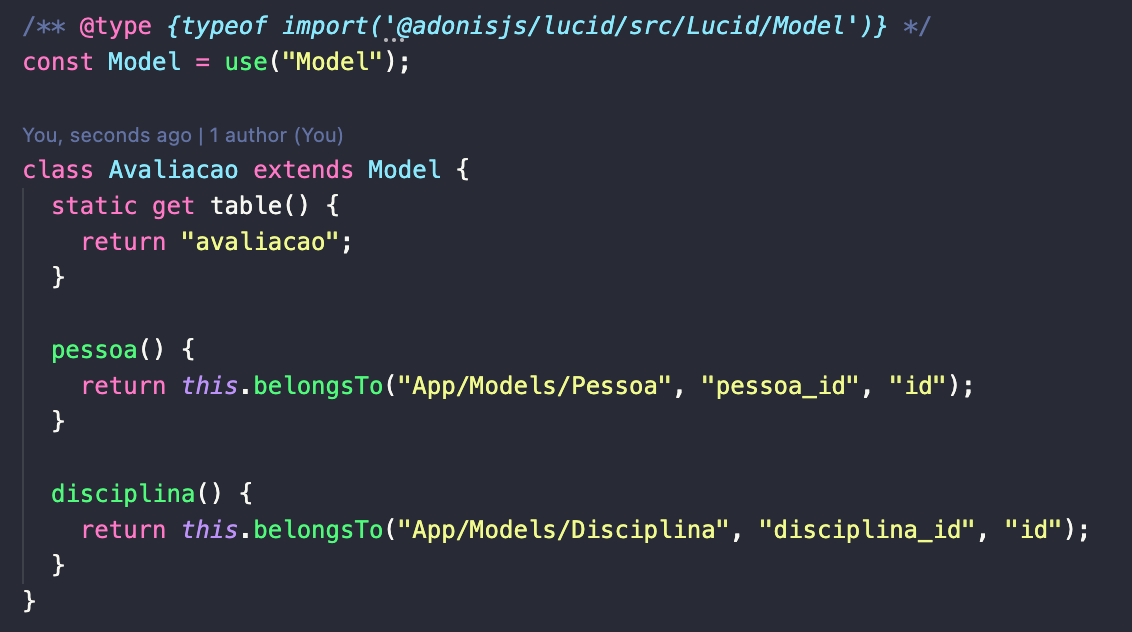
\includegraphics[width=1\textwidth]{imagens/codigo-model-avaliacao.png}
  \caption{Criação do Modelo de Avaliação}
  \label{fig:fig_cod_model_avaliacao}
\end{figure}

\subsection{\textit{Views}}

A camada de \textit{Views}, também conhecida como Visualização, é a responsável por gerar a interface de interação com o usuário. Nessa camada, os dados recebidos do Modelo são processados e apresentados para o usuário da aplicação de maneira interativa. Na arquitetura MVC, a \textit{View} é desacoplada da camada de \textit{Model} e \textit{Controller}, e não possui lógicas de negócio nem interage com a camada de dados.

Para desenvolvimento da camada de Visualização na aplicação proposta utilizamos a biblioteca Bootstrap. A biblioteca disponibiliza classes prontas de CSS, o que facilita a criação de elementos como botões, tabelas e \textit{cards}. Além disso, a biblioteca oferece alguns recursos interativos como \textit{dropdowns} e modais. Com o Bootstap, podemos gerar interfaces com eficiência para renderizar dados de forma compreensível e intuitiva para os usuários.

Dentre as principais \textit{Views} da aplicação está a tela de login, ilustrada na figura \ref{fig:fig_tela_login}. Nessa tela, o usuário pode se autenticar no sistema informando o e-mail e a senha. Caso o usuário não esteja cadastro no sistema ele pode clicar no botão \textbf{Realizar cadastro}, que irá redirecioná-lo para a tela de cadastro ilustrada na figura \ref{fig:fig_tela_cadastro}.

\begin{figure}[h]
  \centering
  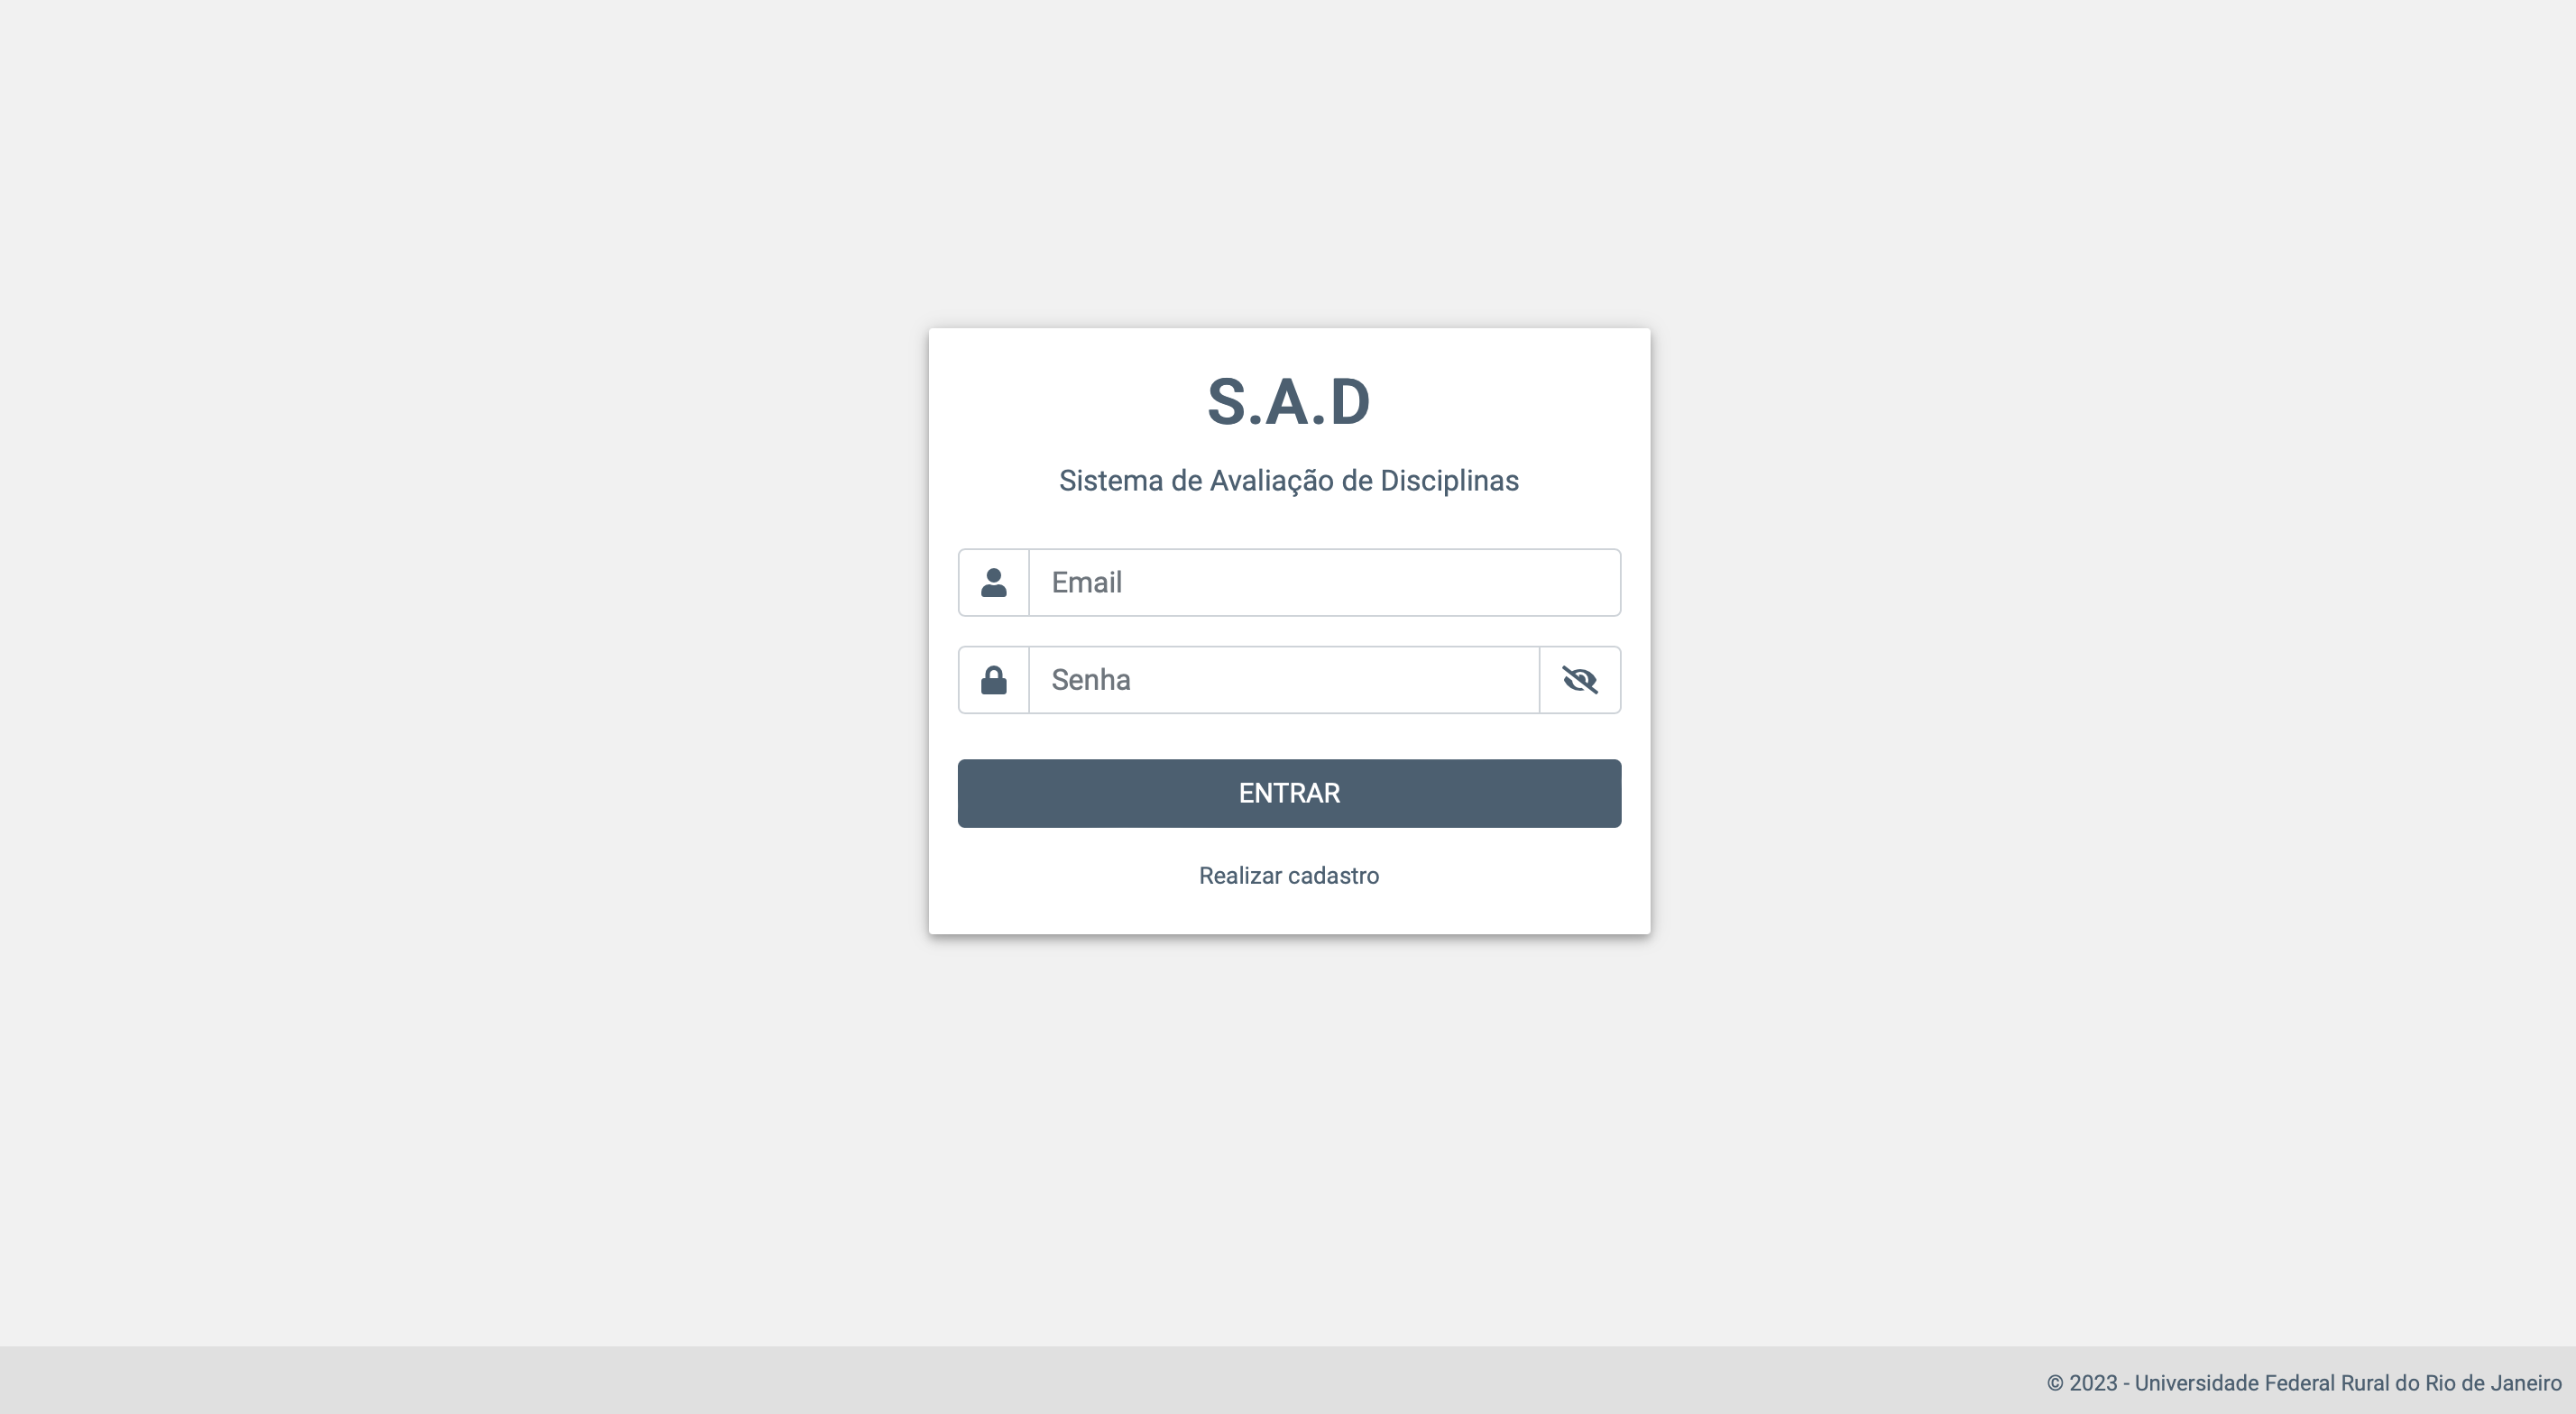
\includegraphics[width=1\textwidth]{imagens/tela-login.png}
  \caption{Tela de login da aplicação proposta}
  \label{fig:fig_tela_login}
\end{figure}

\begin{figure}[!htb]
  \centering
  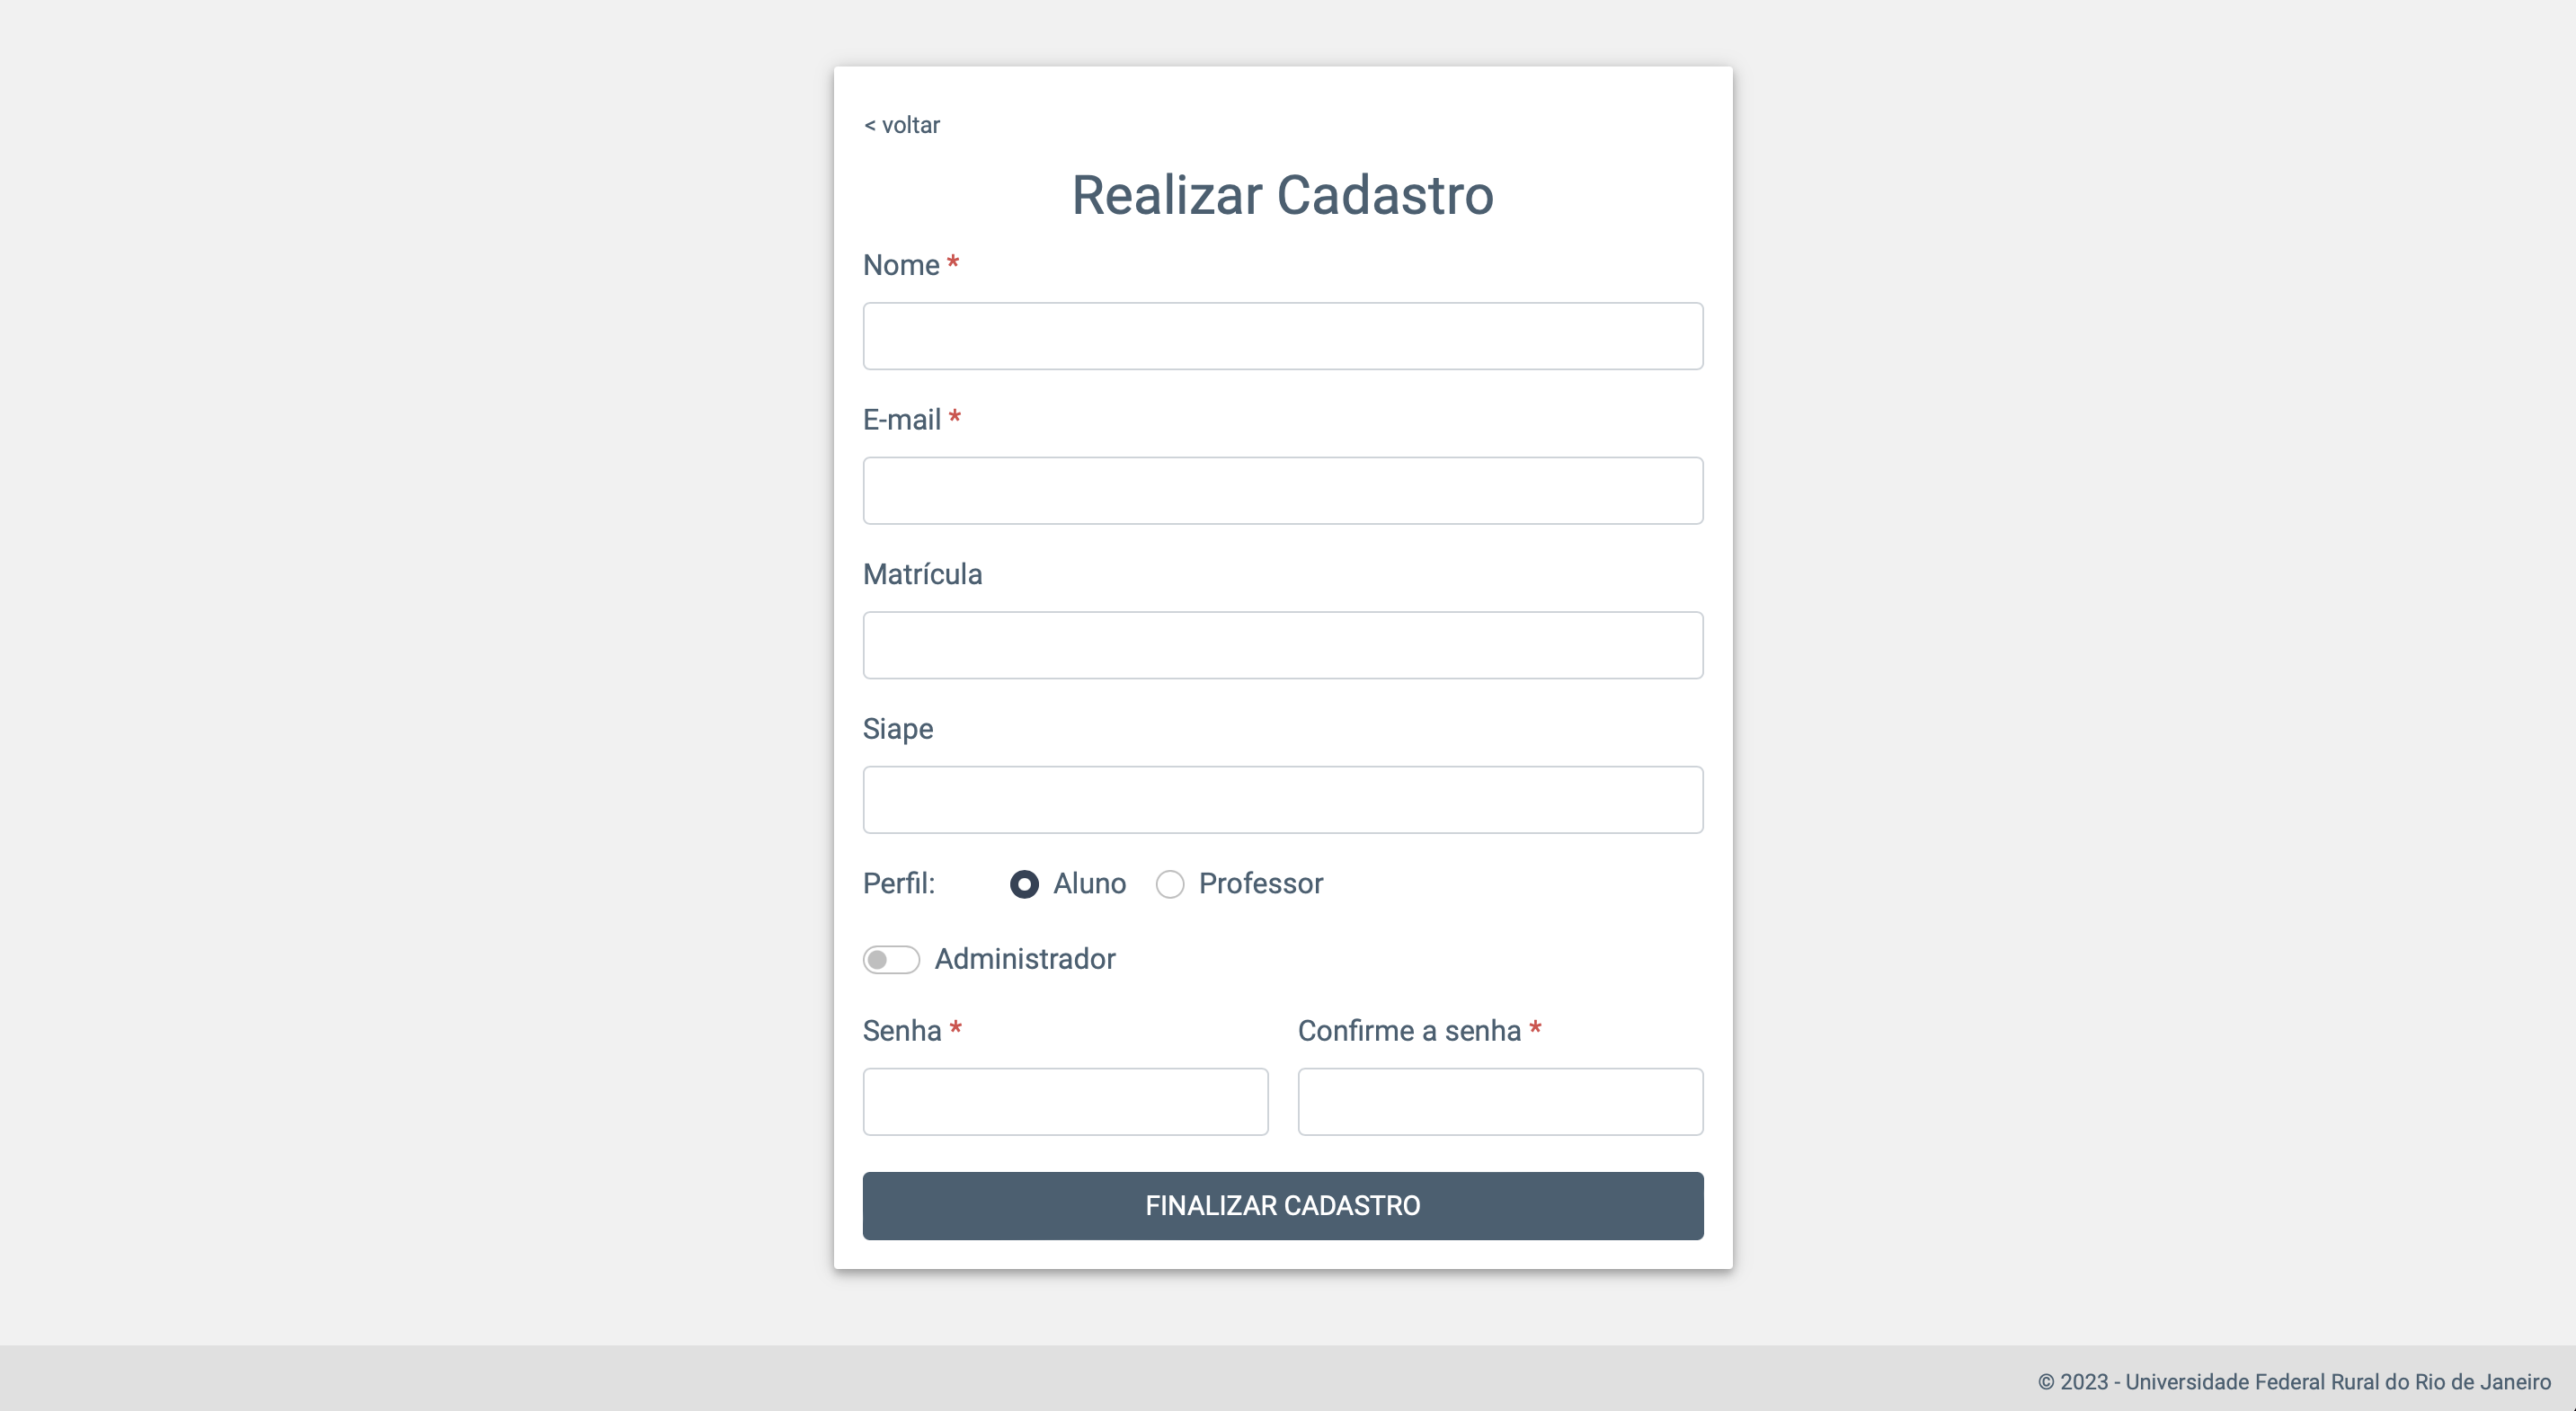
\includegraphics[width=1\textwidth]{imagens/tela-cadastro.png}
  \caption{Tela de cadastro da aplicação proposta}
  \label{fig:fig_tela_cadastro}
\end{figure}

Se o usuário for um Aluno, após se autenticar no sistema ele será redirecionado para a tela de lista de lista de disciplinas como ilustrado na figura \ref{fig:fig_tela_disciplinas_aluno}. Nessa tela, o aluno verá quais disciplinas ainda estão pendentes de avaliação. Caso a disciplina já tenha sido avaliada, o botão \textbf{Avaliar} estará desabilitado.

\begin{figure}[ht]
  \centering
  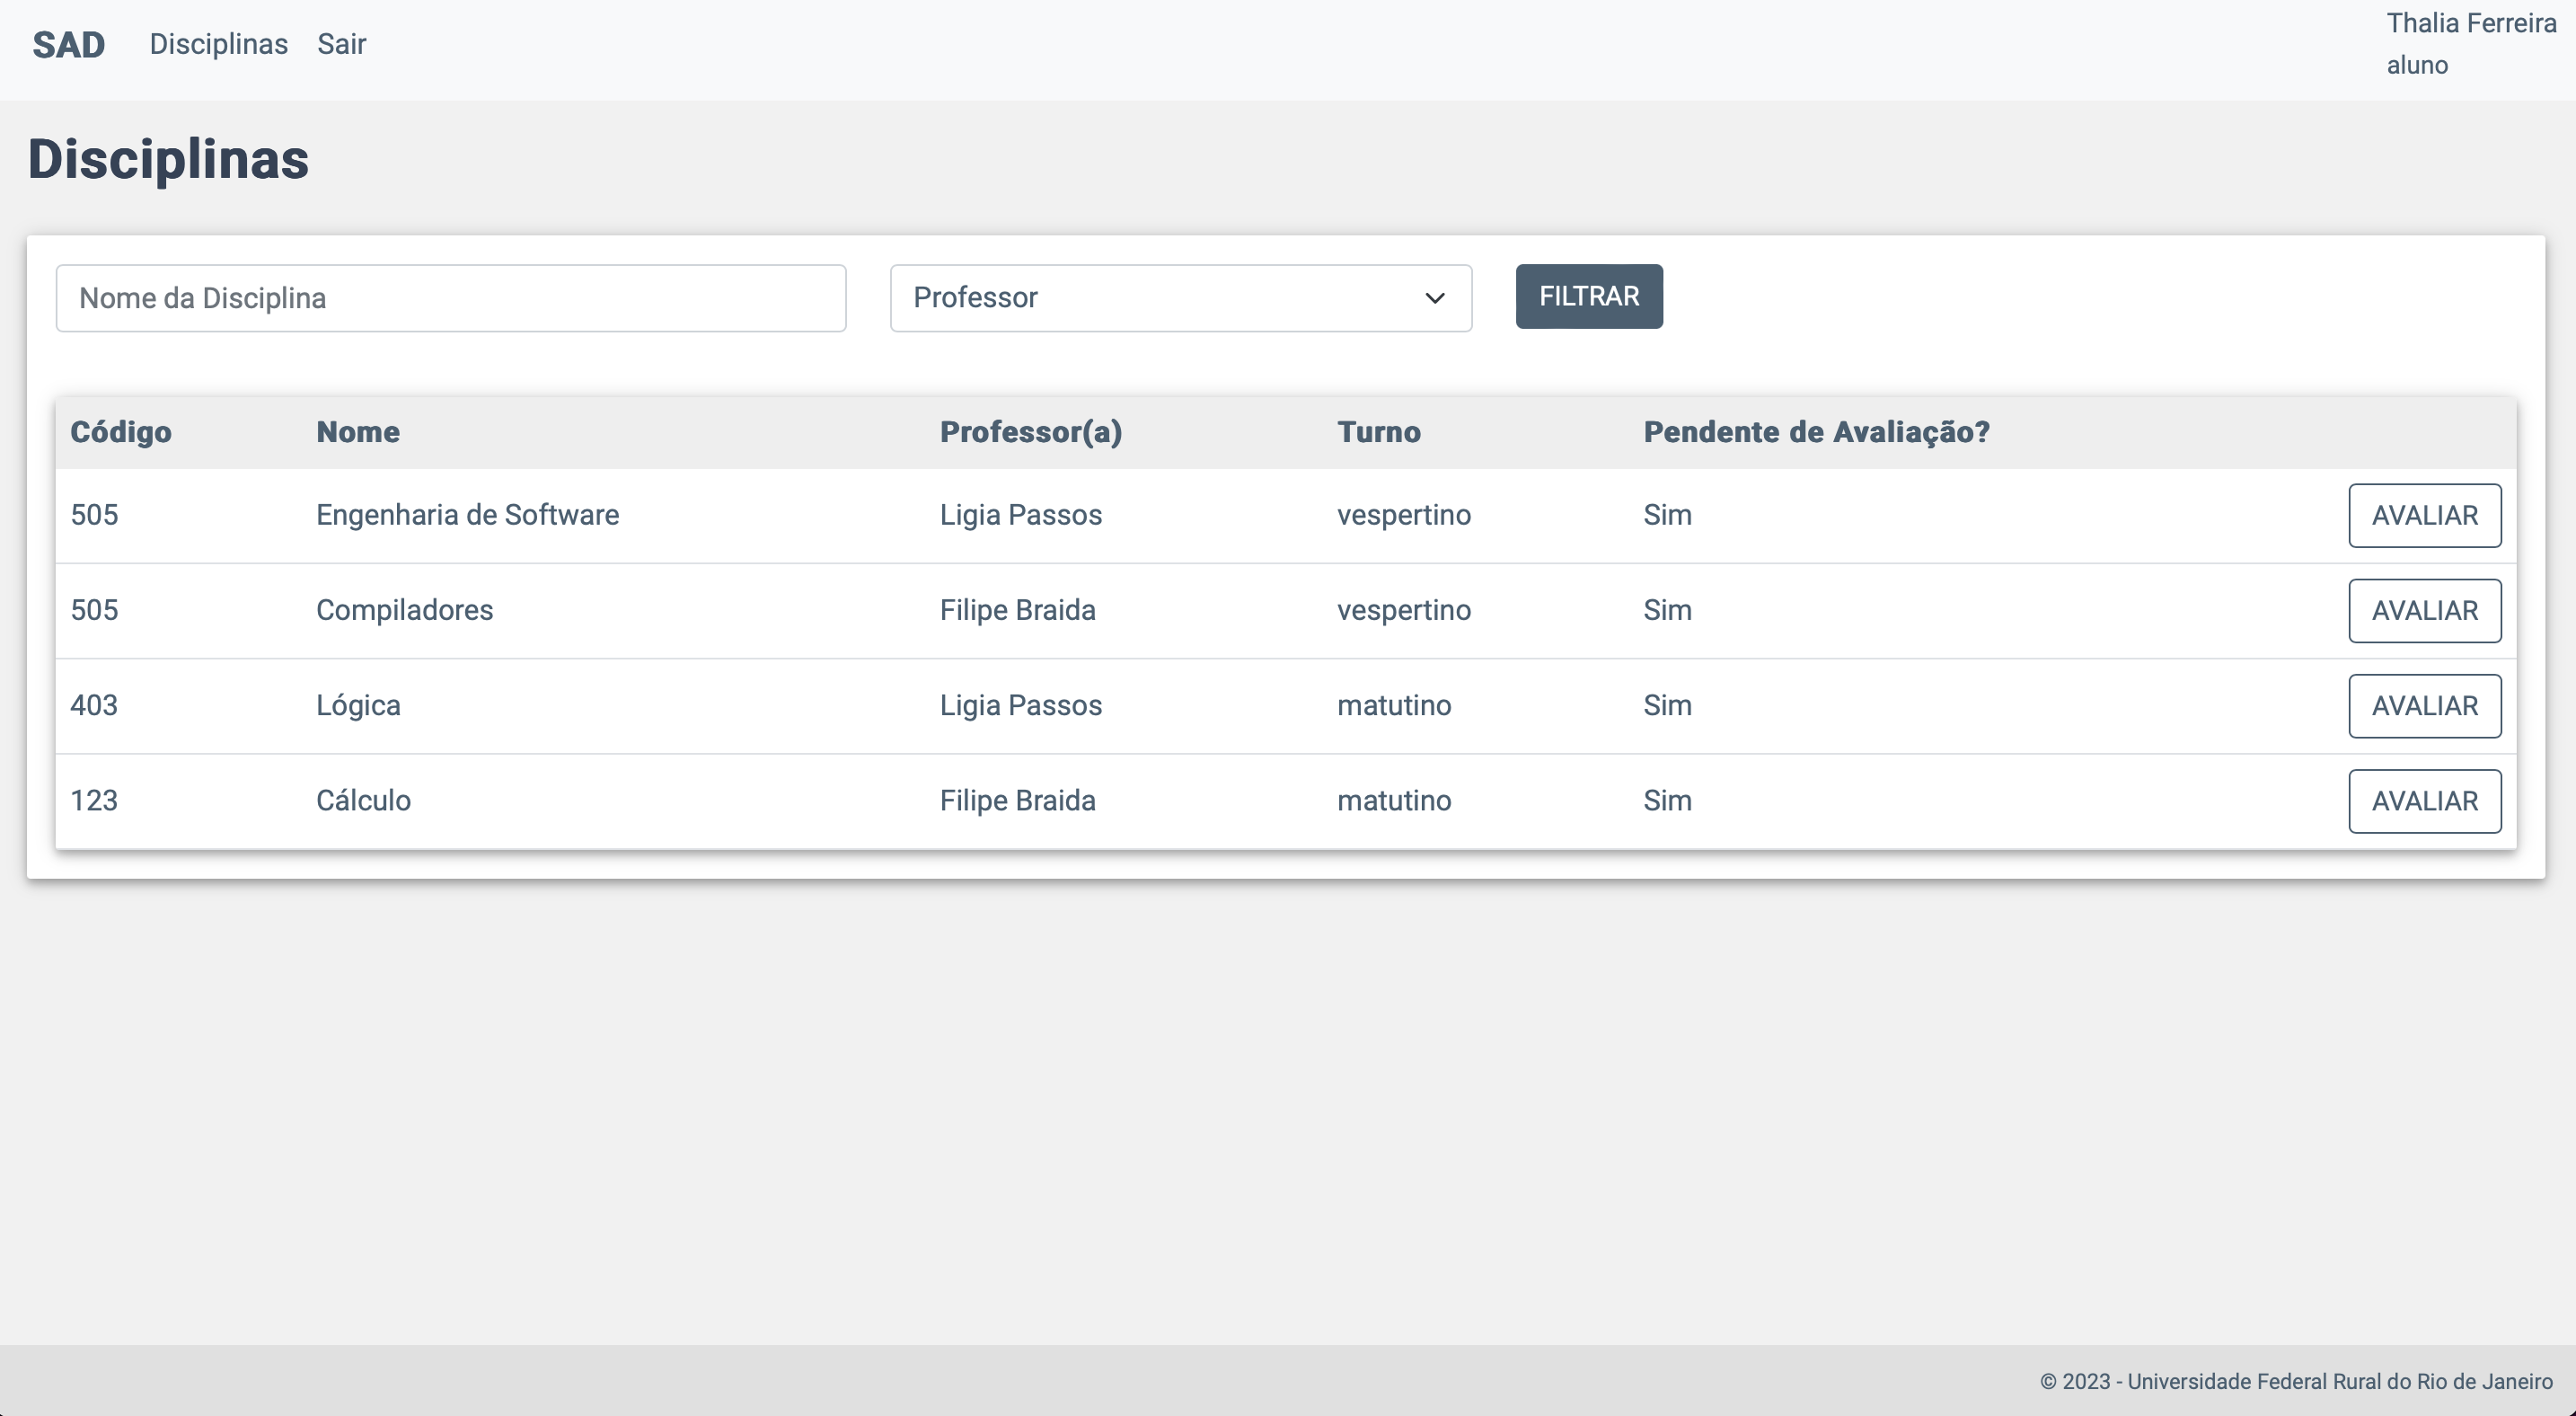
\includegraphics[width=1\textwidth]{imagens/tela-disciplinas-aluno.png}
  \caption{Tela de lista de disciplinas do aluno}
  \label{fig:fig_tela_disciplinas_aluno}
\end{figure}


\subsection{\textit{Controllers}}


\begin{figure}[h]
  \centering
  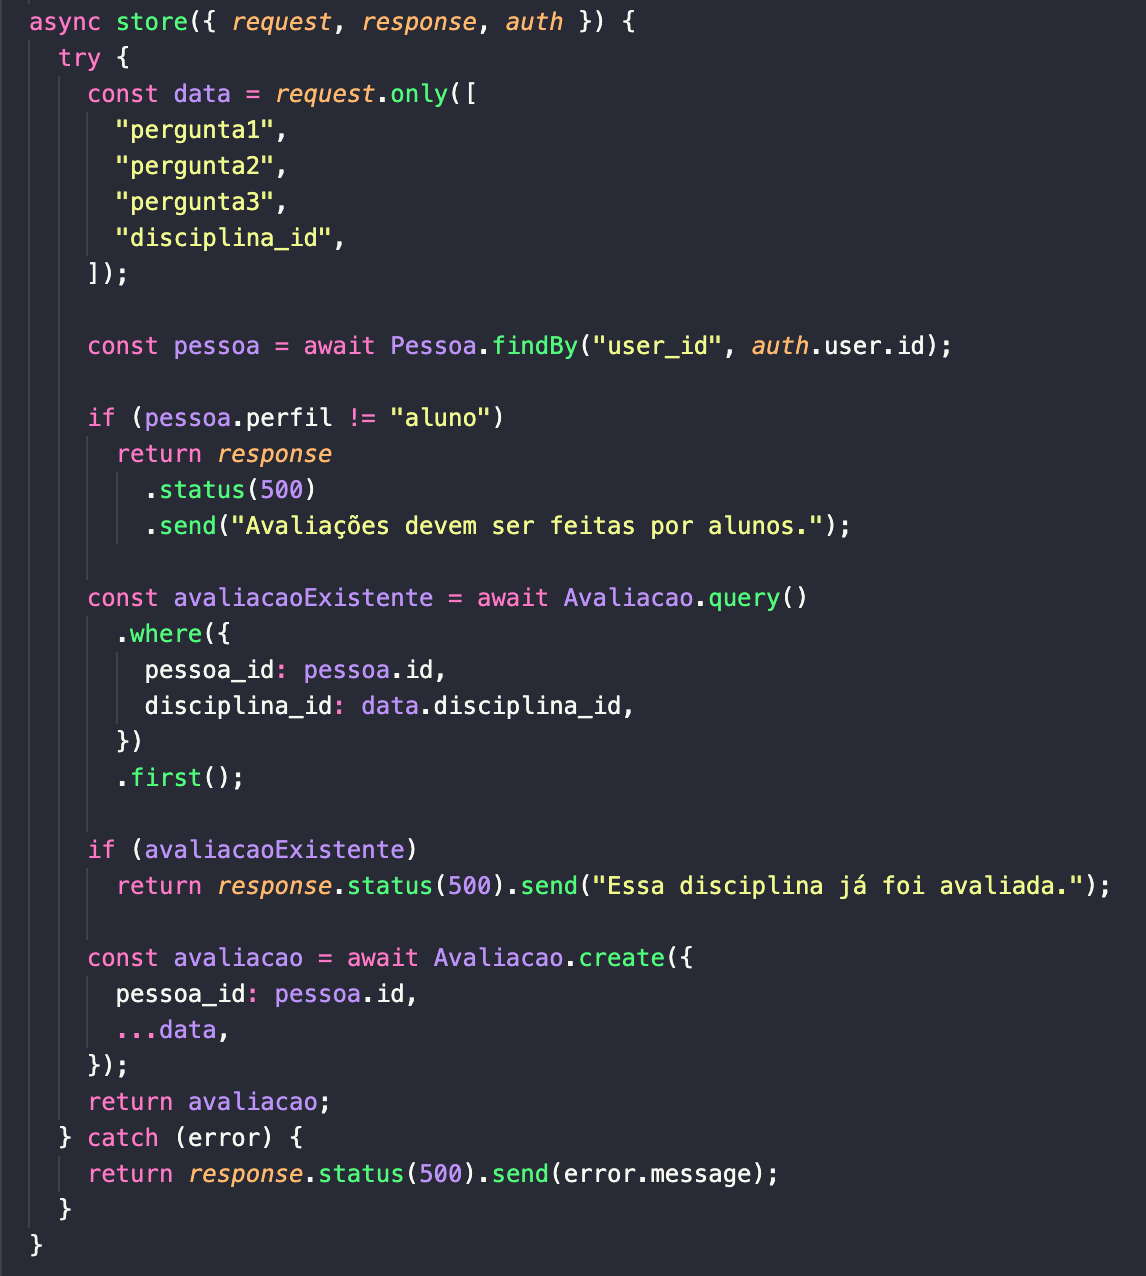
\includegraphics[width=1\textwidth]{imagens/codigo-controller-avaliacao.png}
  \caption{Método de POST na Controller de Avaliação}
  \label{fig:fig_cod_controller_avaliacao}
\end{figure}

\input{elementos-textuais/conclusao}
\pagebreak

%%%%%%%%%%%%%%%%%%%%%%%%%%%%%%%%%%%%%%%%%%%%%%%%%%%%%%%%%%%%
% B I B L I O G R A F I A
%%%%%%%%%%%%%%%%%%%%%%%%%%%%%%%%%%%%%%%%%%%%%%%%%%%%%%%%%%%%
% Retirar esta parte se o trabalho não tiver bibliografia
\makebibspage{elementos-postextuais/referencias}

%%%%%%%%%%%%%%%%%%%%%%%%%%%%%%%%%%%%%%%%%%%%%%%%%%%%%%%%%%%%
% A P E N D I C E
%%%%%%%%%%%%%%%%%%%%%%%%%%%%%%%%%%%%%%%%%%%%%%%%%%%%%%%%%%%%
% Retirar esta parte se o trabalho não tiver anexos
\appendix
\input{elementos-postextuais/apendice}

\end{document}